\centering{\chapter*{Appendix}}
\begin{figure*}[H]
\centering
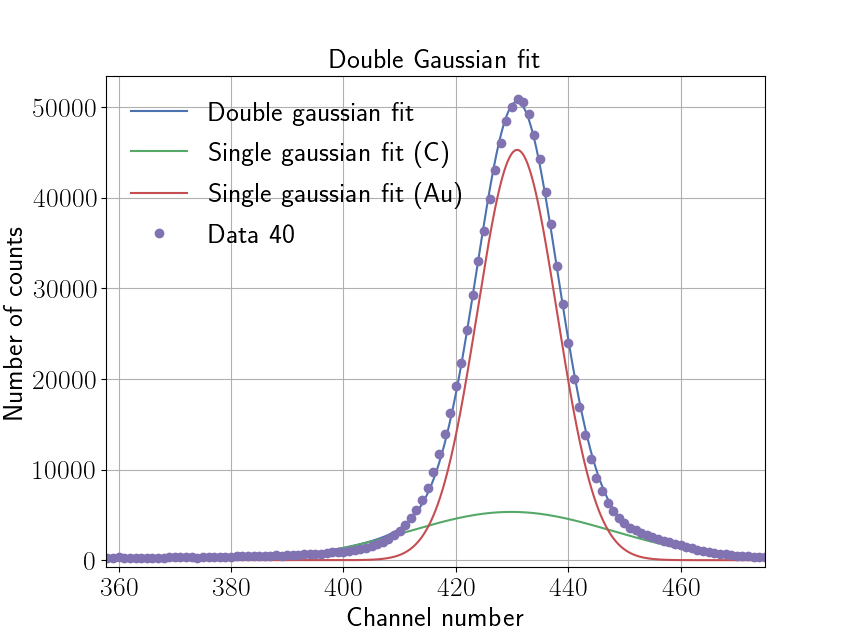
\includegraphics[width=0.99\columnwidth]{Data_40}
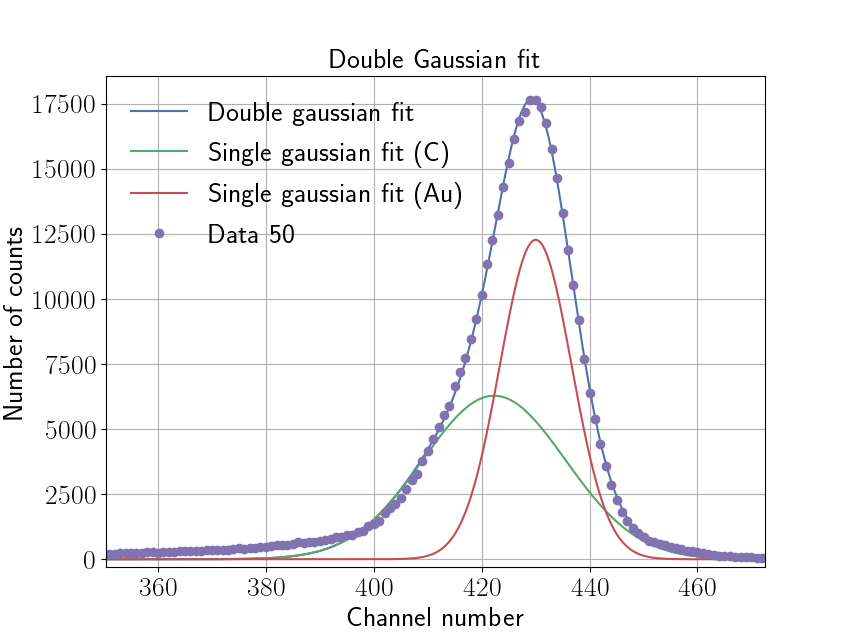
\includegraphics[width=0.99\columnwidth]{Data_50}
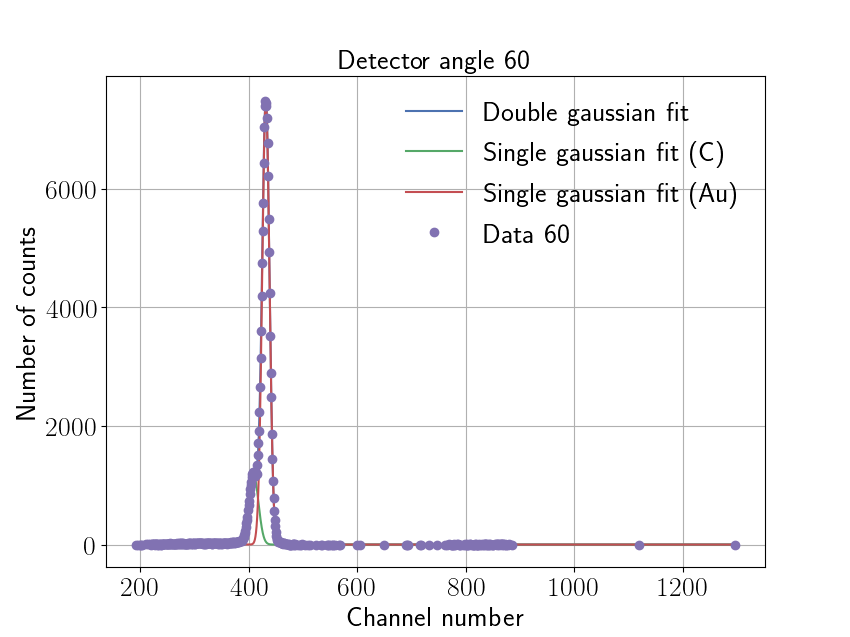
\includegraphics[width=0.99\columnwidth]{Data_60}
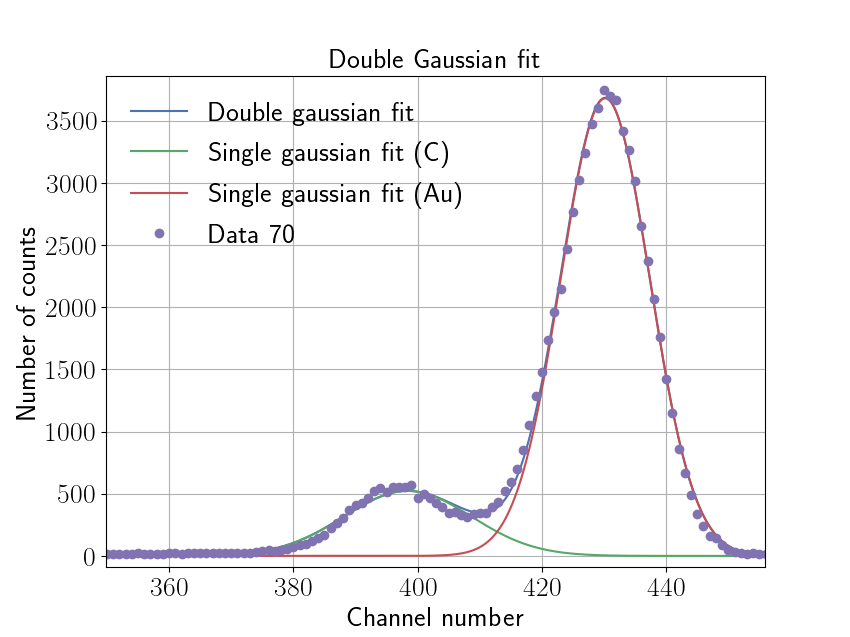
\includegraphics[width=0.99\columnwidth]{Data_70}
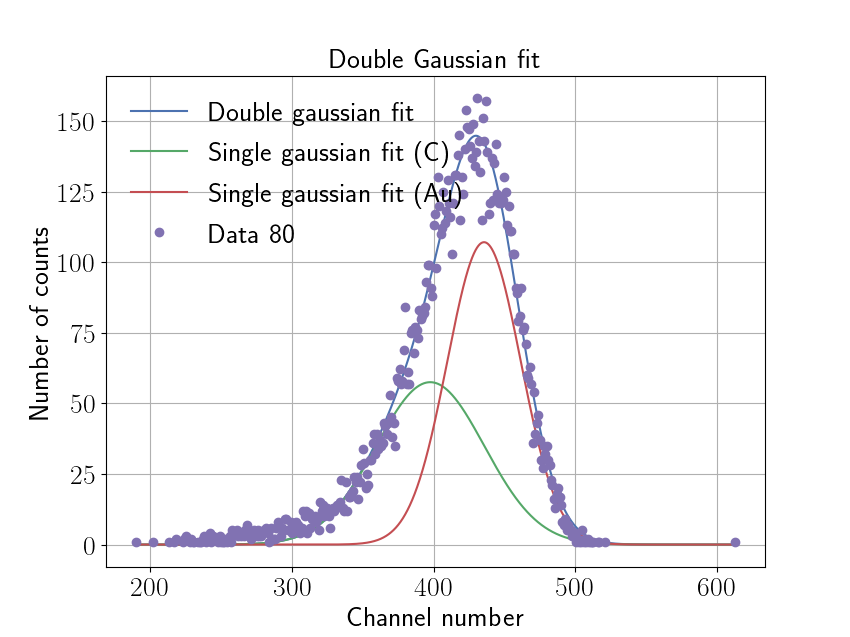
\includegraphics[width=0.99\columnwidth]{Data_80}
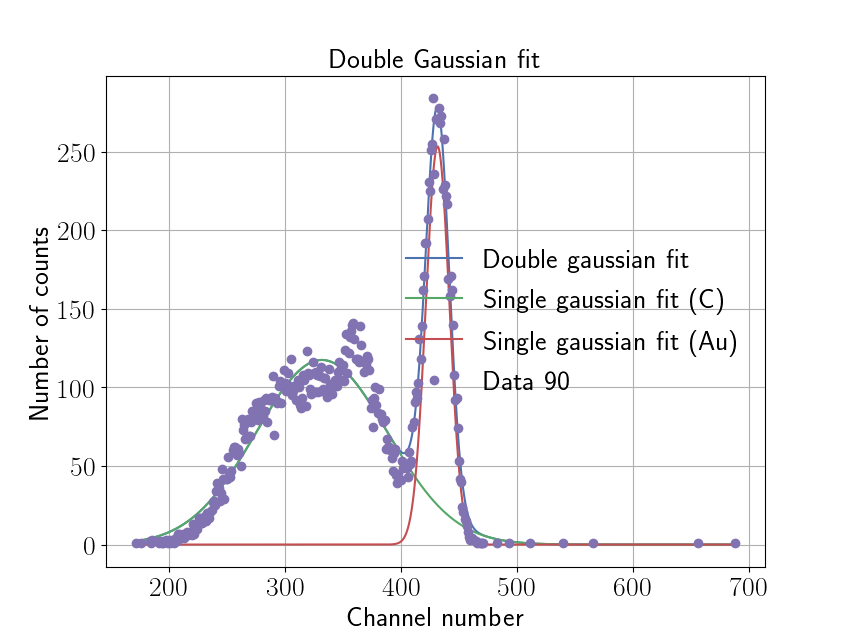
\includegraphics[width=0.99\columnwidth]{Data_90}
%\label{fig_angular_dependency}
\end{figure*}

\newpage
\begin{figure*}
    \centering
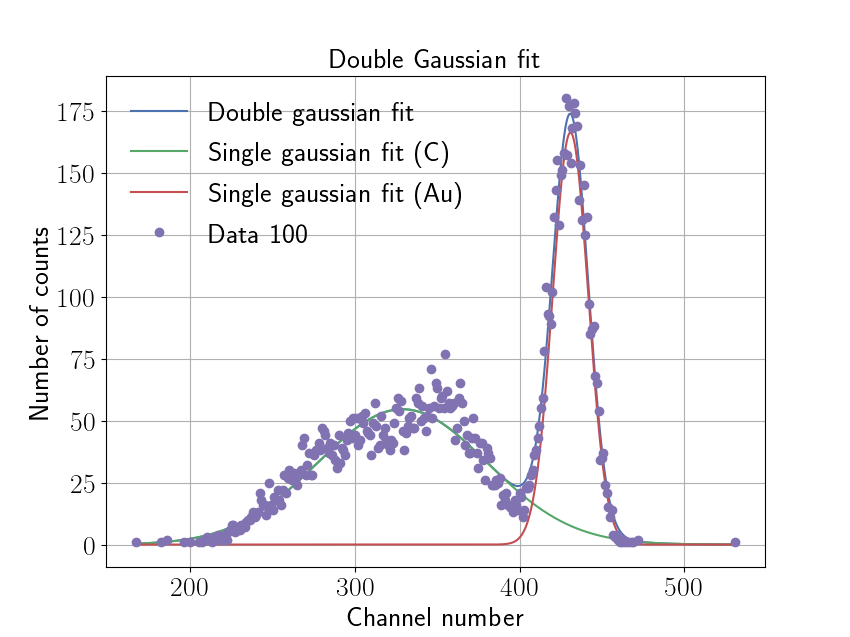
\includegraphics[width=0.99\columnwidth]{Data_100}
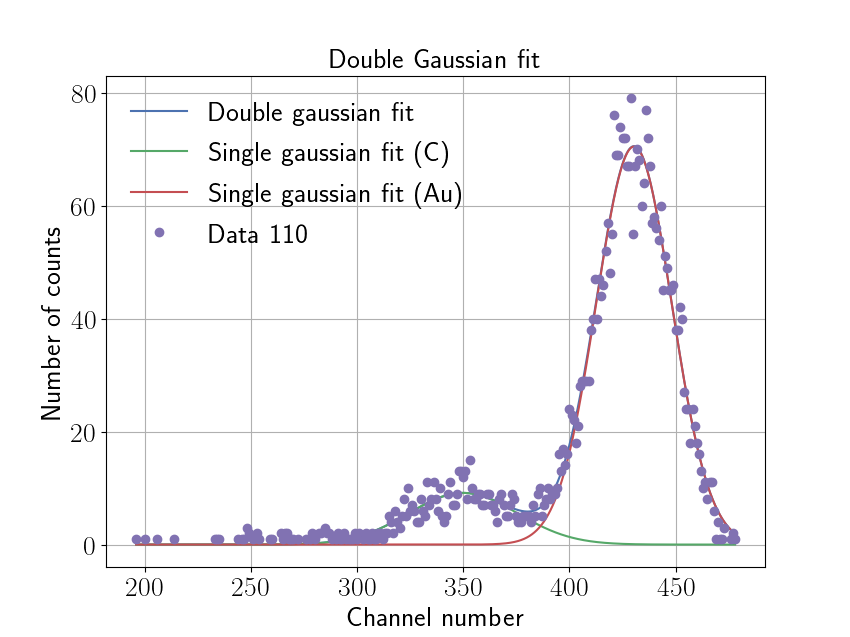
\includegraphics[width=0.99\columnwidth]{Data_110}
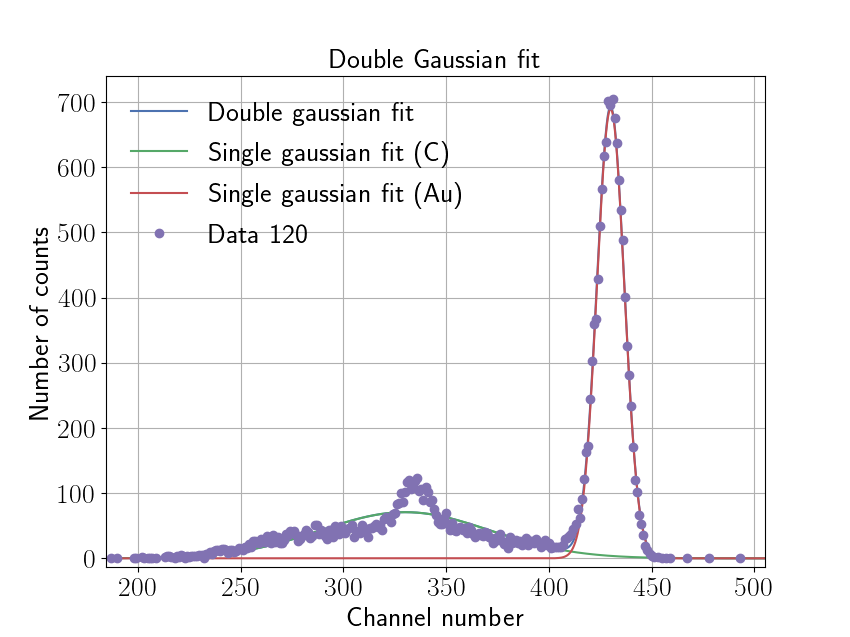
\includegraphics[width=0.99\columnwidth]{Data_120}
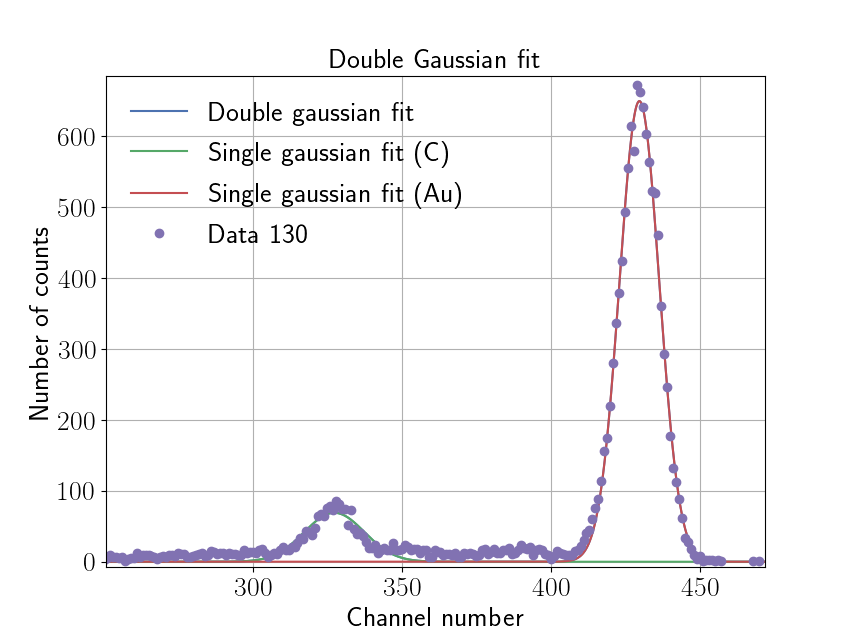
\includegraphics[width=0.99\columnwidth]{Data_130}
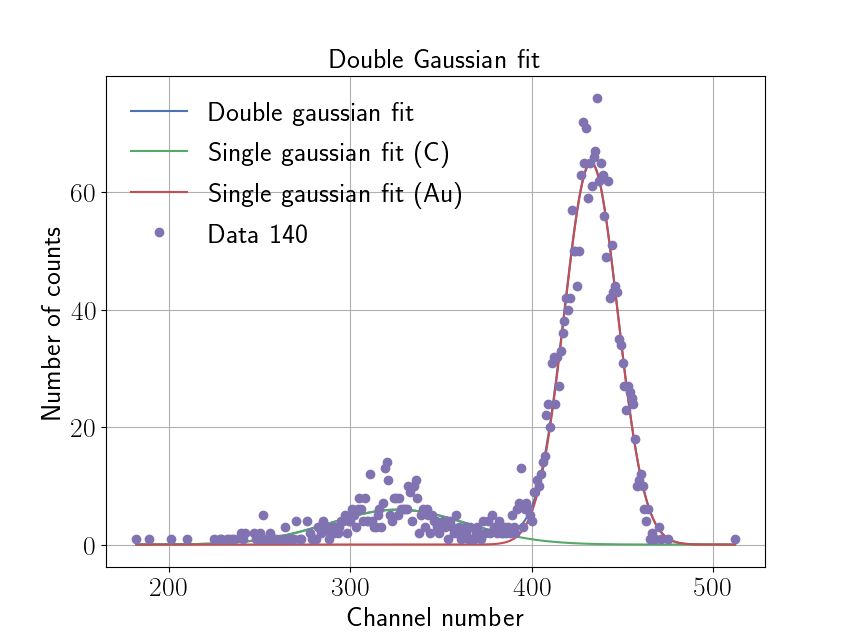
\includegraphics[width=0.99\columnwidth]{Data_140}
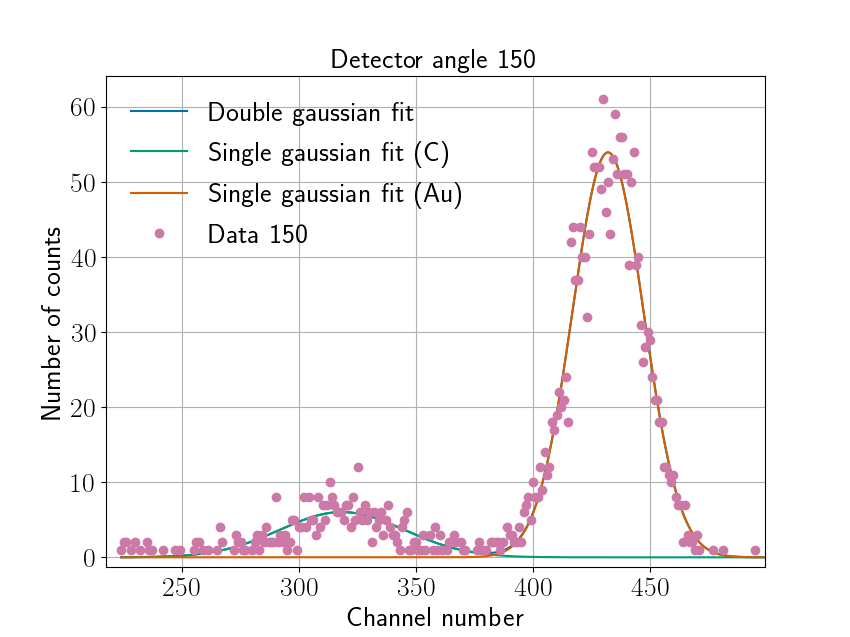
\includegraphics[width=0.99\columnwidth]{Data_150}
\caption{Detected counts at for different scattering angles, and their double gaussian fit.}
\label{fig_angular_dependency}
\end{figure*}
